\subsection{L'usage des scripts}
TODO a revoir ou supprimer
\subsection{L'utilisation de l'interface graphique}

\subsubsection{La fenêtre de choix de taille du rendu}

Lors de l'exécution du main de MainApp on obtient la fenêtre suivante :
\begin{figure}[h]
   \caption{Fênetre de sélection de la taille du rendu}
   \begin{center}
       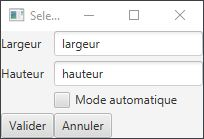
\includegraphics{img/render.javafx/choiceWindow.jpg}
   \end{center}
\end{figure}

Cette fenêtre permet à l'utilisateur de sélectionner la résolution du rendu qu'il souhaite.
Activer le mode automatique maximisera la fenêtre et étendra le rendu sur tout l'écran. Si la résolution sélectionnée est alors inférieure à la résolution de l'écran, la qualité de l'image pourrait s'en trouver altérée.

\subsubsection{La fenêtre d'affichage du rendu}

Une fois que l'utilisateur a entré des paramètres valides, le rendu s'affichera.

Deux fenêtres s'afficheront alors :

\begin{figure}[h]
   \caption{Fenêtre du rendu}
   \begin{center}
       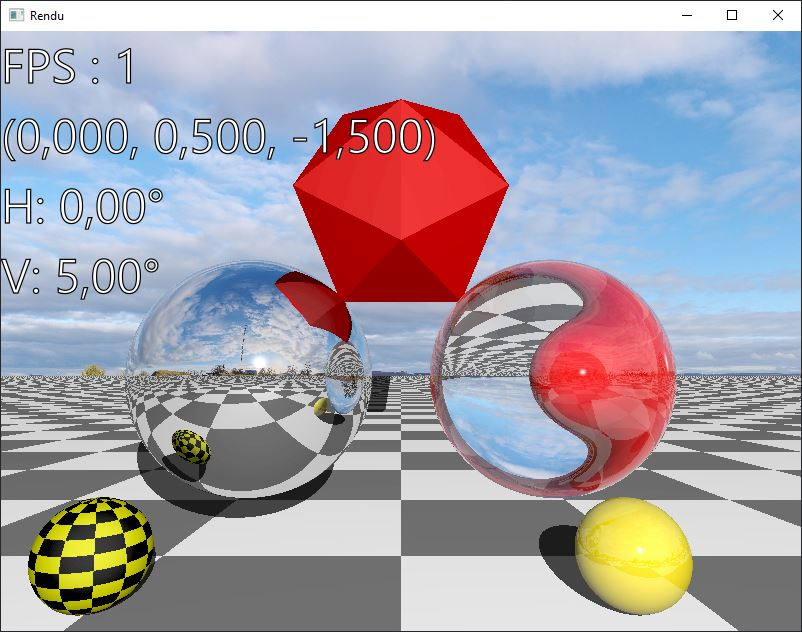
\includegraphics{img/render.javafx/render.jpg}
   \end{center}
\end{figure}

\begin{figure}[h]
   \caption{Fenêtre de la boite à outils}
   \begin{center}
       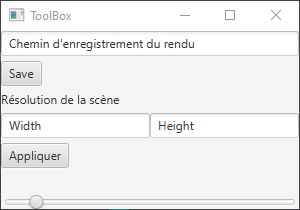
\includegraphics{img/render.javafx/toolbox.jpg}
   \end{center}
\end{figure}
